\documentclass[11pt,oneside]{article}

\pdfminorversion=7
\usepackage{QuizStyle}
\usepackage{tikz}
\usetikzlibrary{positioning}
\tikzset{
    quizvertex/.style={circle,fill=black,inner sep=1.9pt},
    quizedge/.style={line width=0.58pt}
}

\hypersetup{
    pdftitle={20261126 Quiz for MATH261 Discrete Mathematics},
    pdfauthor={Jungwoo Kim},
    pdfsubject={Homework 5 problems and solutions for MATH261 Discrete Mathematics},
    pdfcreator={LaTeX}
}

\begin{document}

\quiztitle{20261126 Quiz}

\begin{problem}{1}
Show that an $n$-vertex simple graph $G$ is connected if
$|E(G)|>\binom{n-1}{2}$.
\end{problem}

\begin{solution}
Suppose that $G$ is disconnected. Choose a connected component with $k$ vertices,
where $1\leq k\leq n-1$. No edge joins this component to the remaining
$n-k$ vertices. Since $G$ is simple,
\[
    |E(G)|\leq\binom{k}{2}+\binom{n-k}{2}
    \leq\binom{n-1}{2}.
\]
The second inequality follows from
\[
    \binom{n-1}{2}-\binom{k}{2}-\binom{n-k}{2}
    =(k-1)(n-k-1)\geq0.
\]
This contradicts the assumption. Hence $G$ is connected.
\end{solution}

\begin{problem}{2}
For each of the following graphs, determine
\begin{problemchoices}[label=(\roman*)]
    \item whether Dirac's Theorem can be used to show that the graph has a Hamiltonian cycle;
    \item whether Ore's Theorem can be used to show that the graph has a Hamiltonian cycle;
    \item whether the graph has a Hamiltonian cycle.
\end{problemchoices}

% The graphs are redrawn from HW5 with identical edge sets.
% (a), (b): a=bottom-left, b=bottom-right, c=top-right,
% d=roof apex, e=top-left. Graph (b) additionally has edge eb.
% (c): a,b,c,d=rectangle corners in clockwise order; e=center.
% (d): a,b,c,d=rectangle corners; e,f=upper/lower inner vertices.
% Coordinates are deliberately symmetric; crossings are not extra vertices.
\begin{center}
\begin{minipage}[t]{0.242\linewidth}\centering
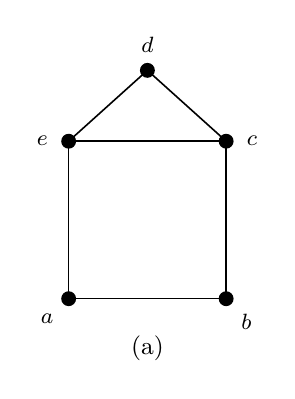
\begin{tikzpicture}[x=1cm,y=1cm]
    \coordinate (a) at (0,0);
    \coordinate (b) at (2,0);
    \coordinate (c) at (2,2);
    \coordinate (d) at (1,2.90);
    \coordinate (e) at (0,2);
    \foreach \u/\v in {a/b,b/c,c/d,d/e,e/a,e/c}{\draw[quizedge] (\u)--(\v);}
    \foreach \v in {a,b,c,d,e}{\node[quizvertex] at (\v) {};}
    \node[font=\footnotesize,below left=2pt and 2pt] at (a) {$a$};
    \node[font=\footnotesize,below right=2pt and 2pt] at (b) {$b$};
    \node[font=\footnotesize,right=4pt] at (c) {$c$};
    \node[font=\footnotesize,above=3pt] at (d) {$d$};
    \node[font=\footnotesize,left=4pt] at (e) {$e$};
    \node[font=\small] at (1,-0.63) {(a)};
    \path[use as bounding box] (-0.42,-0.91) rectangle (2.42,3.29);
\end{tikzpicture}
\end{minipage}\hfill
\begin{minipage}[t]{0.242\linewidth}\centering
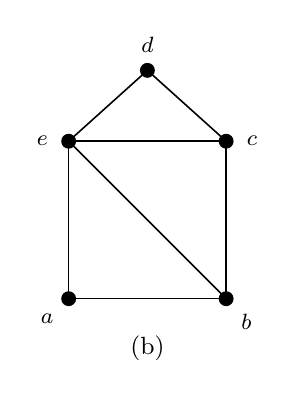
\begin{tikzpicture}[x=1cm,y=1cm]
    \coordinate (a) at (0,0);
    \coordinate (b) at (2,0);
    \coordinate (c) at (2,2);
    \coordinate (d) at (1,2.90);
    \coordinate (e) at (0,2);
    \foreach \u/\v in {a/b,b/c,c/d,d/e,e/a,e/c,e/b}{\draw[quizedge] (\u)--(\v);}
    \foreach \v in {a,b,c,d,e}{\node[quizvertex] at (\v) {};}
    \node[font=\footnotesize,below left=2pt and 2pt] at (a) {$a$};
    \node[font=\footnotesize,below right=2pt and 2pt] at (b) {$b$};
    \node[font=\footnotesize,right=4pt] at (c) {$c$};
    \node[font=\footnotesize,above=3pt] at (d) {$d$};
    \node[font=\footnotesize,left=4pt] at (e) {$e$};
    \node[font=\small] at (1,-0.63) {(b)};
    \path[use as bounding box] (-0.42,-0.91) rectangle (2.42,3.29);
\end{tikzpicture}
\end{minipage}\hfill
\begin{minipage}[t]{0.242\linewidth}\centering
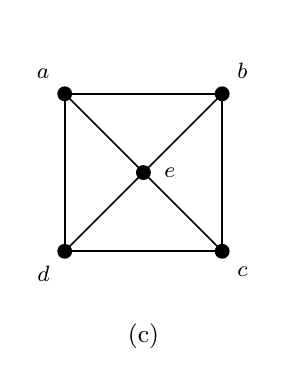
\begin{tikzpicture}[x=1cm,y=1cm]
    \coordinate (a) at (0,2.45);
    \coordinate (b) at (2,2.45);
    \coordinate (c) at (2,0.45);
    \coordinate (d) at (0,0.45);
    \coordinate (e) at (1,1.45);
    \foreach \u/\v in {a/b,b/c,c/d,d/a,a/e,b/e,c/e,d/e}{\draw[quizedge] (\u)--(\v);}
    \foreach \v in {a,b,c,d,e}{\node[quizvertex] at (\v) {};}
    \node[font=\footnotesize,above left=2pt and 2pt] at (a) {$a$};
    \node[font=\footnotesize,above right=2pt and 2pt] at (b) {$b$};
    \node[font=\footnotesize,below right=2pt and 2pt] at (c) {$c$};
    \node[font=\footnotesize,below left=2pt and 2pt] at (d) {$d$};
    \node[font=\footnotesize,right=4pt] at (e) {$e$};
    \node[font=\small] at (1,-0.63) {(c)};
    \path[use as bounding box] (-0.42,-0.91) rectangle (2.42,3.29);
\end{tikzpicture}
\end{minipage}\hfill
\begin{minipage}[t]{0.242\linewidth}\centering
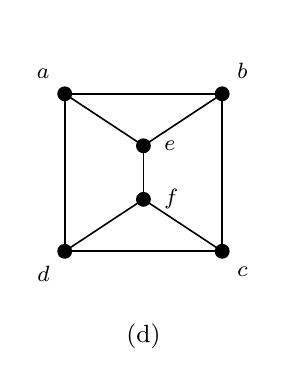
\begin{tikzpicture}[x=1cm,y=1cm]
    \coordinate (a) at (0,2.45);
    \coordinate (b) at (2,2.45);
    \coordinate (c) at (2,0.45);
    \coordinate (d) at (0,0.45);
    \coordinate (e) at (1,1.79);
    \coordinate (f) at (1,1.11);
    \foreach \u/\v in {a/b,b/c,c/d,d/a,a/e,b/e,e/f,d/f,c/f}{\draw[quizedge] (\u)--(\v);}
    \foreach \v in {a,b,c,d,e,f}{\node[quizvertex] at (\v) {};}
    \node[font=\footnotesize,above left=2pt and 2pt] at (a) {$a$};
    \node[font=\footnotesize,above right=2pt and 2pt] at (b) {$b$};
    \node[font=\footnotesize,below right=2pt and 2pt] at (c) {$c$};
    \node[font=\footnotesize,below left=2pt and 2pt] at (d) {$d$};
    \node[font=\footnotesize,right=4pt] at (e) {$e$};
    \node[font=\footnotesize,right=4pt] at (f) {$f$};
    \node[font=\small] at (1,-0.63) {(d)};
    \path[use as bounding box] (-0.42,-0.91) rectangle (2.42,3.29);
\end{tikzpicture}
\end{minipage}
\end{center}
\end{problem}

\begin{solution}
The conditions in Dirac's and Ore's theorems are sufficient, not necessary,
for the existence of a Hamiltonian cycle. The results are
\begin{center}
\begin{tabular}{@{}cccccc@{}}
\toprule
Graph & $|V|$ & $\delta(G)$ & Dirac & Ore & Hamiltonian cycle \\
\midrule
(a) & $5$ & $2$ & No & No & Yes \\
(b) & $5$ & $2$ & No & No & Yes \\
(c) & $5$ & $3$ & Yes & Yes & Yes \\
(d) & $6$ & $3$ & Yes & Yes & Yes \\
\bottomrule
\end{tabular}
\end{center}
For (a) and (b), the vertices $a$ and $d$ are nonadjacent and both have
degree $2$. Thus $\delta(G)=2<5/2$, and
$\deg_G(a)+\deg_G(d)=4<5$; neither theorem applies.

For (c), $\delta(G)=3\geq5/2$, and for (d),
$\delta(G)=3=6/2$. Hence Dirac's Theorem applies in both cases.
Ore's condition also holds: any two distinct nonadjacent vertices have
sum of degrees at least $2\delta(G)\geq|V(G)|$.

To verify Hamiltonicity directly in every case, the labeled drawings give
Hamiltonian cycles
\[
\begin{aligned}
\text{(a), (b):}\quad & a-b-c-d-e-a,\\
\text{(c):}\quad & a-b-c-e-d-a,\\
\text{(d):}\quad & a-b-c-d-f-e-a.
\end{aligned}
\]
In particular, (a) and (b) are Hamiltonian even though neither theorem
can establish this.
\end{solution}

\begin{problem}{3}
Dirac's Theorem cannot be extended to the condition $\delta(G)<n/2$:
some graphs satisfying this inequality are Hamiltonian, while others are not.
Give an example of a non-Hamiltonian graph satisfying $\delta(G)<n/2$.
\end{problem}

\begin{solution}
Consider the star graph $G=K_{1,3}$, which has $4$ vertices and
$\delta(G)=1<4/2$. Its three leaves each have degree $1$, whereas every
vertex of a Hamiltonian cycle must be incident to two edges of that cycle.
Thus $G$ is not Hamiltonian.
\end{solution}

\begin{problem}{4}
\begin{problemsubparts}
    \item For every $n\geq2$, find a non-Hamiltonian graph on $n$ vertices
    with $\binom{n-1}{2}+1$ edges.
    \item For every $n\geq2$, find a non-Hamiltonian graph on $n$ vertices
    with minimum degree $\lceil n/2\rceil-1$.
\end{problemsubparts}
\end{problem}

\begin{solution}
\begin{problemsubparts}
\item Start with $K_{n-1}$ and add a new vertex $v$ adjacent to exactly one
existing vertex. The resulting graph has $n$ vertices and
\[
    |E(G)|=\binom{n-1}{2}+1.
\]
Since $\deg_G(v)=1$, it has no Hamiltonian cycle. This construction also
works when $n=2$.

\item For $n=2$, take the graph consisting of two isolated vertices;
its minimum degree is $0=\lceil2/2\rceil-1$, and it is not Hamiltonian.

For $n\geq3$, set
\[
    G=K_{\lceil n/2\rceil-1,\,\lfloor n/2\rfloor+1}.
\]
The two parts have different sizes and together contain $n$ vertices.
Their sizes give
\[
    \delta(G)=\lceil n/2\rceil-1.
\]
Every cycle in a bipartite graph alternates between its two parts,
so a Hamiltonian cycle would have to use equally many vertices from
each part. This is impossible here; hence $G$ is not Hamiltonian.
\end{problemsubparts}
\end{solution}

\begin{problem}{5}
Use Ore's Theorem to give a short proof that any graph $G$ on $n$ vertices
with more than $\binom{n-1}{2}+1$ edges has a Hamiltonian cycle.
\end{problem}

\begin{solution}
The hypothesis is impossible for $n\leq2$, so assume $n\geq3$.
Let $u,v$ be any two distinct nonadjacent vertices. Since $uv\notin E(G)$,
all edges either lie among the other $n-2$ vertices or are incident to $u$
or $v$. Therefore,
\[
    |E(G)|\leq\binom{n-2}{2}+\deg_G(u)+\deg_G(v).
\]
By the hypothesis,
\[
    \deg_G(u)+\deg_G(v)
    \geq |E(G)|-\binom{n-2}{2}
    >n-1.
\]
As the degrees are integers, $\deg_G(u)+\deg_G(v)\geq n$.
Thus Ore's condition holds for every pair of distinct nonadjacent vertices,
so $G$ is Hamiltonian.
\end{solution}

\begin{remark}
The construction in Problem 4(a) has exactly
$\binom{n-1}{2}+1$ edges and is not Hamiltonian, showing that the
edge threshold in Problem 5 is sharp.
\end{remark}

\end{document}
